% Document class and basic setup
\documentclass[10pt]{exam}
% \usepackage[utf8]{inputenc}
% \usepackage[T1]{fontenc}

% Page layout and geometry
\usepackage[margin=0.25in, includefoot, includehead]{geometry}
\usepackage{microtype}

% Font packages - XeLaTeX/LuaLaTeX vs pdfLaTeX compatibility
\usepackage{ifxetex,ifluatex}
\ifxetex
\usepackage{fontspec}
\setmainfont{Linux Libertine O}[
  Ligatures=TeX,
  Numbers=OldStyle
]
\setsansfont{Linux Biolinum O}[
  Ligatures=TeX,
  Numbers=OldStyle
]
% \setmonofont{Latin Modern Mono}[Scale=MatchLowercase]
\setmonofont{DejaVu Sans Mono}[Scale=MatchLowercase]
\else\ifluatex
\usepackage{fontspec}
\setmainfont{Linux Libertine O}[
  Ligatures=TeX,
  Numbers=OldStyle
]
\setsansfont{Linux Biolinum O}[
  Ligatures=TeX,
  Numbers=OldStyle
]
\setmonofont{Latin Modern Mono}[Scale=MatchLowercase]
\else
\usepackage{libertine}
\fi\fi

% Math packages
\usepackage{amsmath,amssymb,amsthm}
\usepackage{mathtools}
\usepackage{bm}
\usepackage{accents}

% List and enumeration
\usepackage[shortlabels]{enumitem}
\usepackage{multicol}

% Graphics and figures
\usepackage{graphicx}
\usepackage{tikz}
\usepackage{pgfplots}
\pgfplotsset{compat=1.18}
\usetikzlibrary{shapes}
\usepackage{pgfplots}
\pgfplotsset{compat=1.18}
% \usepackage{svg}
\usepackage{graphicx}
\usepackage{float}
\usepackage{wrapfig}

% Tables and arrays
\usepackage{booktabs}
\usepackage{multirow}
\usepackage{nicematrix}

% Color and highlighting
\usepackage{xcolor}
\definecolor{answerboxcolor}{RGB}{255,245,245} % Very light red background
\usepackage{empheq}
\usepackage{ulem}

% Captions and references
\usepackage[hypcap=false,font=small,labelfont=bf,tableposition=top]{caption}
\usepackage{subcaption}
\usepackage[colorlinks=true, linkcolor=blue, urlcolor=blue]{hyperref}
\usepackage{cleveref}

% Units and chemistry
\usepackage{siunitx}
\sisetup{
  group-digits=integer,
  group-minimum-digits=3,
  group-separator={,}
}
\DeclareSIUnit\angstrom{\text{\AA}} % \angstrom is depracted, so define it here.
\usepackage[version=4]{mhchem}
\usepackage{chemformula}

% Code listings
\usepackage{minted}
\usepackage{listings}
\AtBeginEnvironment{minted}{
\fontsize{8}{10}\selectfont}

% Utility packages
\usepackage{cancel}
\usepackage{etoolbox}
\usepackage{pdfpages}
\usepackage{blindtext}
\usepackage{lipsum}

% Custom commands
\newcommand{\fahrenheit}{^\circ{F}}
\newcommand*\widefbox[1]{\fbox{\hspace{2em}#1\hspace{2em}}}
\newcommand{\msout}[1]{\text{\sout{$#1$}}}

% SI Units
\DeclareSIUnit\year{y}

% Professional boxed answer environment
% Creates uniform, centered answer boxes with light red background
\newcommand{\boxedanswer}[1]{
  \begin{center}
    \fcolorbox{black}{answerboxcolor}{%
      \begin{minipage}{0.85\textwidth}
        \vspace{0.5em}
        #1
        \vspace{0.5em}
      \end{minipage}%
    }
  \end{center}
  \vspace{0.5em}
}

% Alternative boxed answer for nested environments (like enumerate)
\newcommand{\boxedanswersmall}[1]{
  \begin{center}
    \fcolorbox{black}{answerboxcolor}{%
      \begin{minipage}{0.75\textwidth}
        \vspace{0.3em}
        #1
        \vspace{0.3em}
      \end{minipage}%
    }
  \end{center}
  \vspace{0.3em}
}

% Additional SI unit for Fahrenheit
\DeclareSIUnit\fahrenheit{\degree F}

\begin{document}

% Include title page
% Title page with no headers/footers
\thispagestyle{empty}

\begin{titlepage}
  \begin{center}
    \vspace*{2cm}

    % Main title
    \Huge
    \textbf{Homework \#5}

    \vspace{0.8cm}

    % Course information
    \LARGE
    MSEN 640-600

    \vspace{2cm}

    % Author information
    \Large
    \textbf{Prepared by:}\\[0.5cm]
    \huge
    \textbf{Nathaniel Thomas}

    \vspace{1cm}

    \Large
    \textbf{Prepared for:}\\[0.5cm]
    \large
    Dr. Michael Dimitriyev

    \vfill

    % University logo
    
\includegraphics[width=0.4\textwidth]{"./assets/a&m_logo.pdf"}

    \vspace{1cm}

    % University and date information
    \Large
    Materials Science \& Engineering\\
    Texas A\&M University\\
    \vspace{0.5cm}
    \large
    October 28\textsuperscript{th}, 2025

  \end{center}
\end{titlepage}

% Header and footer setup using exam class commands
% The exam class provides its own header/footer system
\lhead{\textbf{MSEN 640-600}}
\chead{\textbf{Homework \#5}}
\rhead{\textbf{Nathaniel Thomas}}
\lfoot{}
\cfoot{\thepage}
\rfoot{}

% Add header rule
\headrule


\pagebreak

\begin{enumerate}
    \item 
        \begin{enumerate}[a.]
            \item (5 points) How many possible microstates exist for a system containing eight atoms of element
            A and one atom of element B? Draw all possible microstates for such a system on a three-by-three
            two-dimensional lattice.
            \item (5 points) How many possible microstates exist for a system containing four atoms of element A,
            two atoms of element B, and three atoms of element C?
        \item (5 points) The following lattices show microstates of a 4x4 lattice. Which is the most probable
            microstate consistent with the macrostate of being \SI{50}{\percent} occupied. Explain your answer.
        \end{enumerate}

    \begin{figure}[h]
        \centering
        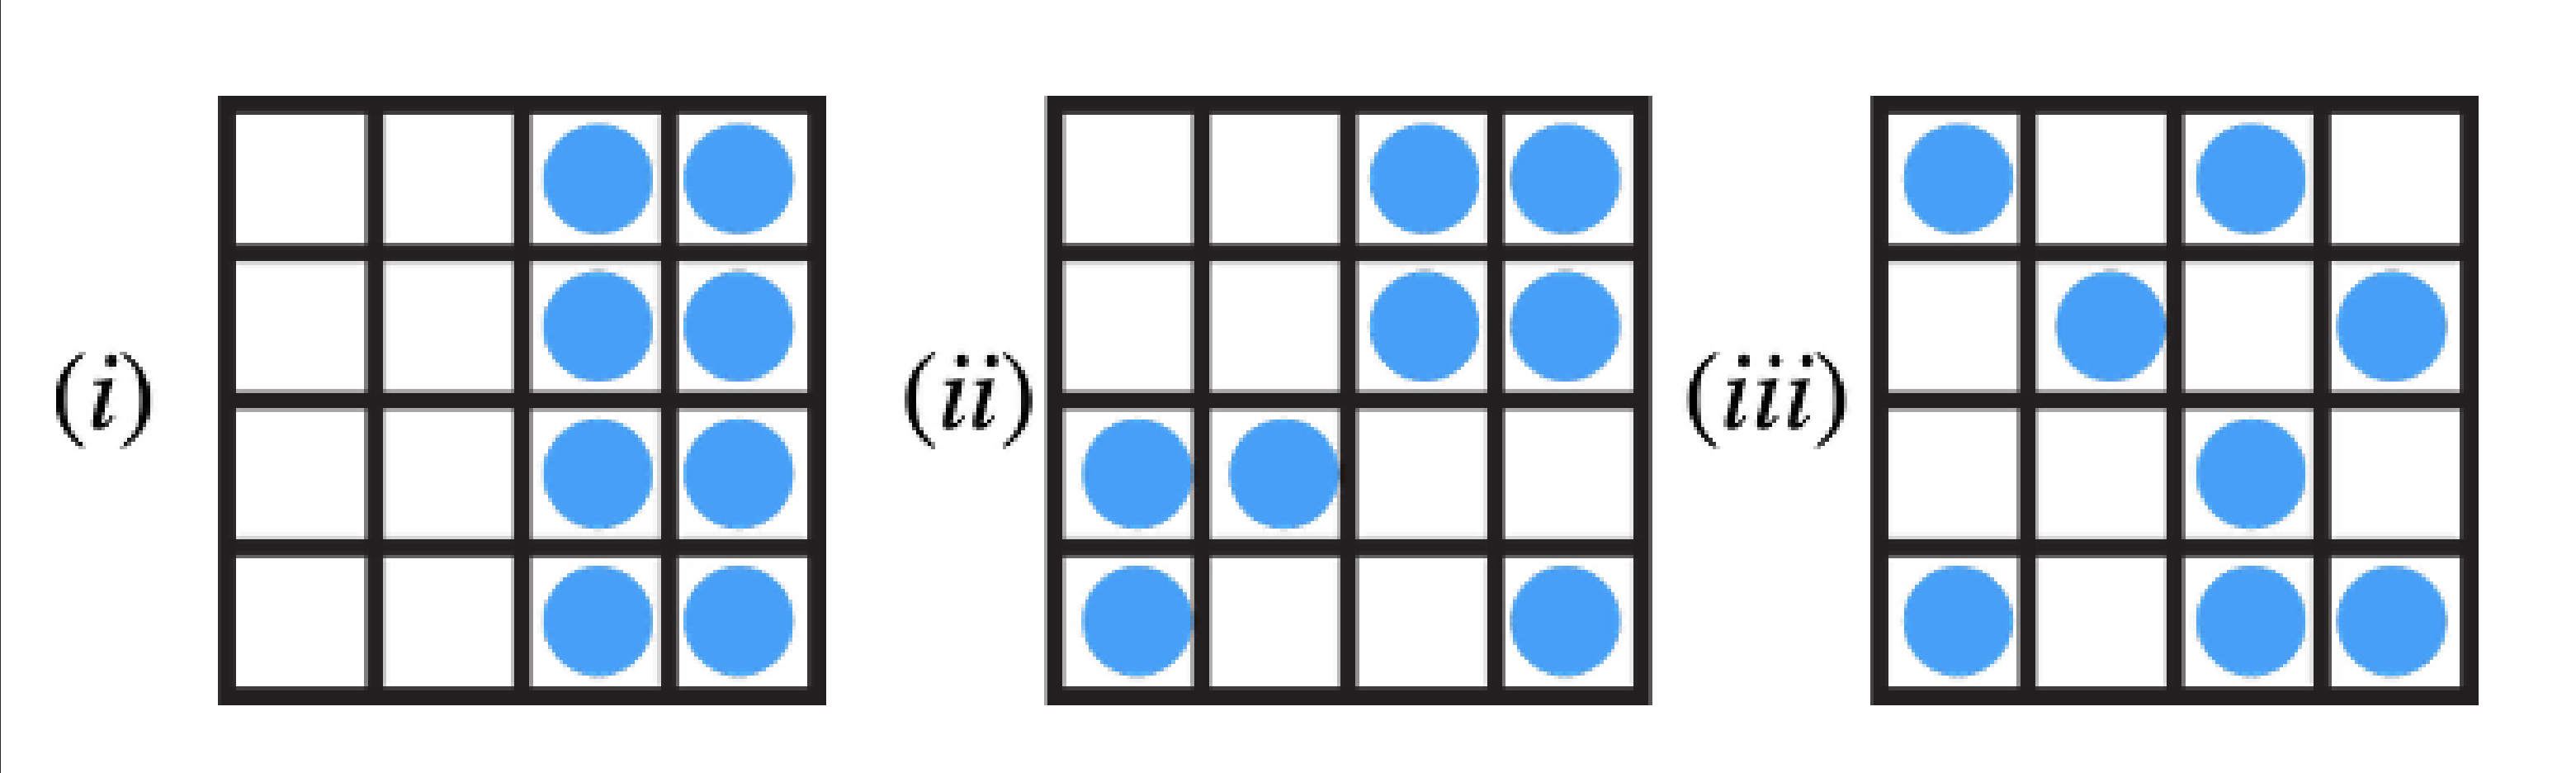
\includegraphics[width=0.6\textwidth]{./assets/fig_1.png}
    \end{figure}

    \pagebreak

    \item Consider a small colloidal glass bead of mass m in a container of water held at temperature $T$. The
    gravitational potential energy $U$ of the glass particle depends on its height above the bottom of the
    container z: $U(z) = mgz$, where $g$ is the acceleration due to gravity.

    \begin{enumerate}
        \item Determine the probability $P(z)$ that the bead is found at a certain height $z$. Normalize the
            probability distribution such that $\int_0^\infty P(z) = 1$.
        \item Calculate the average height of the bead $\langle z\rangle$. Under what conditions would we expect particles
            to “sediment” out of a solution?
        \item In the high temperature limit (or $T \rightarrow \infty$), where can we expect to find the bead? \label{c}
        \item Calculate the variance of the bead height $\langle z^2\rangle - \langle z\rangle^2$. \label{d}
        \item Given what we have learned in part \ref{d}, re-interpret your answer to part \ref{c}. That is, at any
            instant in time, where might the bead be found at high temperatures?
        \item Calculate the average energy $\langle U \rangle$.
    \end{enumerate}
    
    \pagebreak

    \item One simple model of a crystal consists of a collection of masses and springs. Consider one particular
        “normal mode” of the crystal, characterized by natural frequency $\omega$. The vibrational energy associated
        with this normal mode can be quantized such that the $n$\textsuperscript{th} energy level is given by

    \begin{equation*}
        \epsilon_n = \left(n + \frac{1}{2}\right)\hbar \omega
    \end{equation*}


    where $n = 0, 1, 2, \dots$ and $\hbar$ is Planck’s constant divided by $2\pi$. This is called the “Einstein model”
    of a crystalline solid.

    \begin{figure}[h]
        \centering
        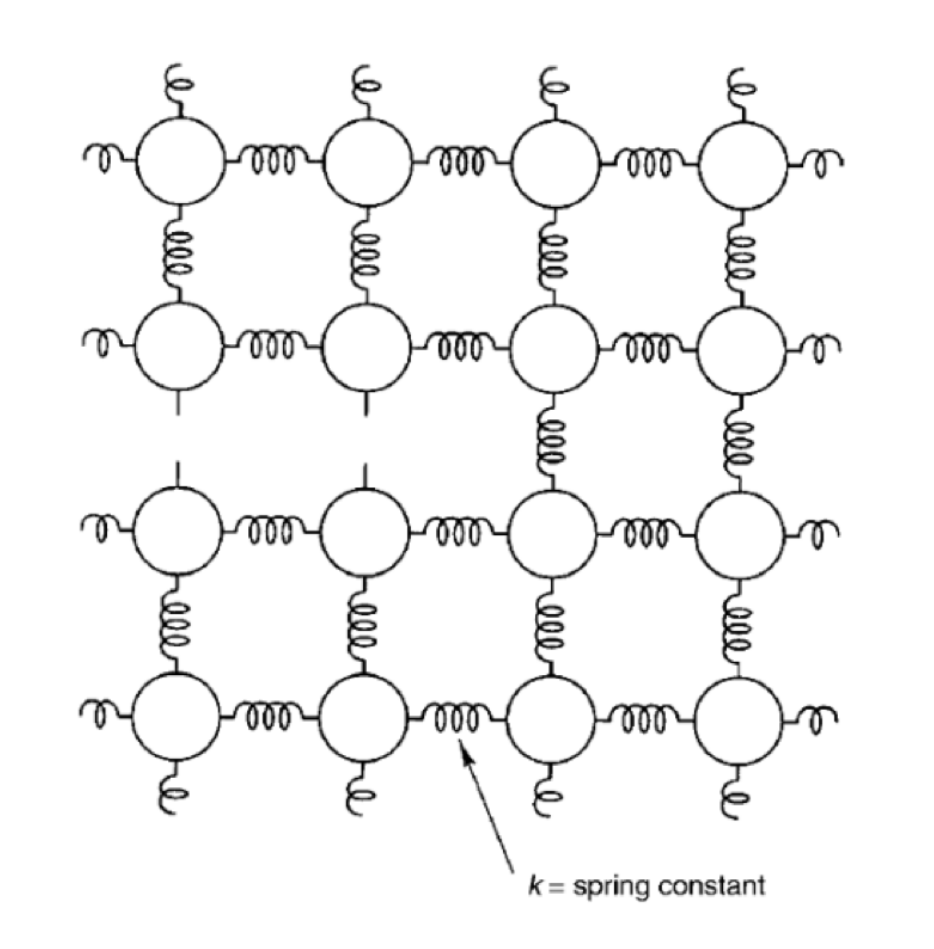
\includegraphics[width=0.4\textwidth]{./assets/fig_2.png}
    \end{figure}
    
    \begin{enumerate}[(a)]

        \item Calculate the partition function $Z$. To simplify, take advantage of the formula for a convergent
            geometric series:

        \begin{equation*}
            \sum_{n=0}^\infty x^n = \frac{1}{1 - x}
        \end{equation*}

        \item Calculate the entropy, internal energy, and Helmholtz free energy of the crystal. 
            You can express your results in terms of the “Einstein temperature” $\vartheta_E  ≡ \hbar \omega/k_B$. 
            (Note that for diamonds, $\vartheta_E \approx \SI{1320}{K}$.)

        \item Calculate the molar heat capacity $C_V$ . Plot $C_V /k_B$ as a function of $T /\vartheta_E$. (This model actually
            does a good job at capturing the high-temperature behavior of real crystals! The low-temperature
            requires some corrections, however.)
    \end{enumerate}




    
\end{enumerate}

% \section*{Supporting code:}
% \inputminted{julia}{./calculations/src/calculations.jl}

\end{document}
